\chapter {Дополнение}

\subsection*{Составить ER-диаграмму (нотацию Чена) для лабораторной работы.}

\begin{figure}[h]
	\centering
	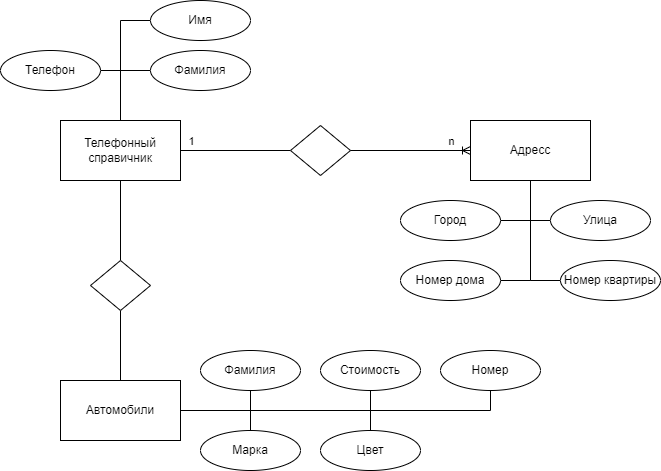
\includegraphics[width=0.85\textwidth]{img/er.png}
	\label{fig:er}
\end{figure}

\clearpage

\subsection*{Привести вопрос и ответ на РЕЯ, Prolog и SQL.}

РЕЯ:

\noindent\begin{minipage}[T]{.5\textwidth}
	\begin{lstlisting}[caption=Вариант 1]
Найти фамилию, город, номер владельца по марки и цвету автомобиля (всех).				
	\end{lstlisting}
\end{minipage}\hfill
\begin{minipage}[T]{.5\textwidth}
	\begin{lstlisting}[caption=Вариант 2]
Найти марку и цвет автомобиля по  фамилии, городу, номеру владельца (всех).	
	\end{lstlisting}
\end{minipage}

Prolog:

\noindent\begin{minipage}[T]{.5\textwidth}
	\begin{lstlisting}[caption=Вариант 1]
predicates
	phone_record(surname, name, address, phone_list).
	car(surname, name, brand, colour, price, car_number).
	question(surname, city, phone_list, brand, colour).
clauses
	question(Surname, City, Phone, Brand, Colour) :-
	phone_record(Surname, _, address_data(City, _, _, _), Phone),
	car(Surname, _, Brand, Colour, _, _).
goal
	question(Surname, City, Phone, "Mercedes", "black").		
	\end{lstlisting}
\end{minipage}\hfill
\begin{minipage}[T]{.5\textwidth}
	\begin{lstlisting}[caption=Вариант 2]
predicates
	phone_record(surname, name, address, phone_list).
	car(surname, name, brand, colour, price, car_number).
	question(surname, city, phone_list, brand, colour).
clauses
	question(Surname, City, Phone, Brand, Colour) :-
	phone_record(Surname, _, address_data(City, _, _, _), Phone),
	car(Surname, _, Brand, Colour, _, _).
goal
question("Иванов", "Новосибирск", ["8456372"], Brand, Colour).
	\end{lstlisting}
\end{minipage}

\clearpage

SQL:

\noindent\begin{minipage}{.5\textwidth}
	\begin{lstlisting}[caption=Вариант 1, language=sql]
SELECT record.surname, record.phone, address.city
FROM car as c join phone_record as pr ON c.surname = pr.surname
JOIN address as ad ON pr.surname = ad.surname
WHERE c.brand = "Mercedes" AND c.colour = "black"		
	\end{lstlisting}
\end{minipage}\hfill
\begin{minipage}{.5\textwidth}
	\begin{lstlisting}[caption=Вариант 2, language=sql]
SELECT c.mark, c.color
FROM auto FROM car as c join phone_record as pr ON c.surname = pr.surname
JOIN address as ad ON pr.surname = ad.surname
WHERE pr.surname = "Иванов" AND pr.phone_list = ["8456372"] AND ad.city = "Новосибирск"
	\end{lstlisting}
\end{minipage}